% !TEX root = SegwayDoku.tex
\newpage
\renewcommand{\autoren}{Valentyn Chepil}
\section{Die Hindernis umfahren}

Die benötigten, reaktiven Fähigkeiten ”Hindernis umfahren”, (bzw. ”Hindernis rechts umfahren” und ”Hindernis links umfahren”) können alternativ mithilfe der Regelungstechnik und zweier grundlegender Teilschritte realisiert werden. Der prinzipielle Ablauf der reaktiven Fähigkeit ist in Abbildung \ref{bild_HUR} dargestellt. 

\begin{figure}[!h]  % [h] bedeutet, dass das Bild genau an dieser Stelle im Text erscheint
	\centering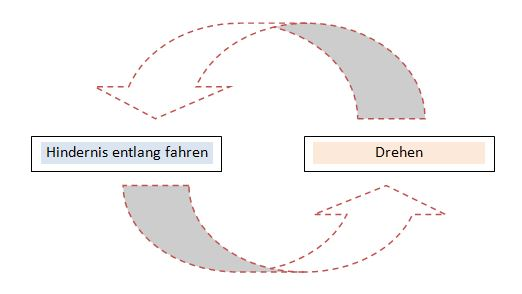
\includegraphics[width=0.6\textwidth]{images/Bild-HUR.jpg}
	\caption{ \ Regelkreis "Hindernis umfahren" (Quelle:Eigene Darstellung)}
	\label{bild_HUR} % über das label kann man aus dem Text auf das Bild verweisen
\end{figure}

In der Abbildung sind zwei prinzipielle Teilschritte abgebildet und durch zwei Farben gekennzeichnet. Zuerst soll sich der Glied in Bezug auf das Hindernis entscheiden, siehe Teilschritt ”Fallauswahl” - Bild \ref{baum2} , anschließend entlang des Hindernisses fahren. Diese beiden Teilschritte werden noch weiter unterteilt. Der Schritt Drehen wird je nach vorgegebener Richtung in ”Drehen rechts” und ”Drehen links” aufgeteilt. Dieser Teilschritt wird als vorgegebene Konstante realisiert und da als Winkel (0 Grad, positiv oder negativ) definiert. ”Hindernis entlang fahren” wird in die Teilschritte "Hindernis rechts entlang Fahren" und "Hindernis links entlang Fahren". Dieser Teilschritt wird als vorgegebene Konstante realisiert

\subsection{Ampelsysten}

Es wurde drei Zone (grün, gelb, rot) von mir definiert, die sich wie "Ampelsysten"  (Abbildung \ref{zone}) verhalten. Im grünen Bereich fährt den Roboter mit voller Geschwindigkeit \textcolor{green}{\textit{skal\_zone=1}}. Bei Erkennung des Hindernis in gelber Zone bremst dem Roboter langsam ab \textcolor{green}{\textit{skal\_zone=0.4}} und fängt manövrieren \textcolor{green}{\textit{drehwinkel=0 Grad, positiv oder negativ}}. Die Geschwindigkeit  des Roboters in roter Zone geht auf 0 \textcolor{green}{\textit{skal\_zone=0}}. Den Roboter im Stillstand sucht als weiterer Schritt einen freien Weg zum Ziel über Teilprogramm "Fallauswahl". In der Abbildung \ref{baum2} ist zu sehen.

Aus der Fähigkeiten des US-Sensors wurde folgende Entfernung in einzelner Zonen definiert:
\begin{figure}[!h]  % [h] bedeutet, dass das Bild genau an dieser Stelle im Text erscheint
	\centering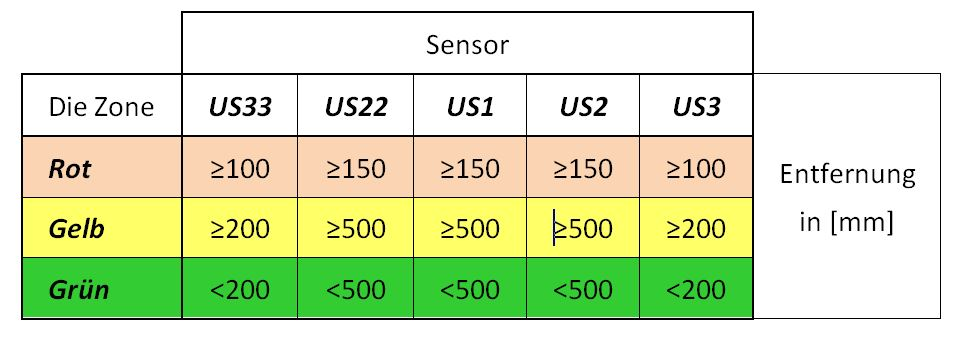
\includegraphics[width=0.60\textwidth]{images/entf.jpg}
	\label{entf} % über das label kann man aus dem Text auf das Bild verweisen
\end{figure}

\begin{figure}[!h]  % [h] bedeutet, dass das Bild genau an dieser Stelle im Text erscheint
	\centering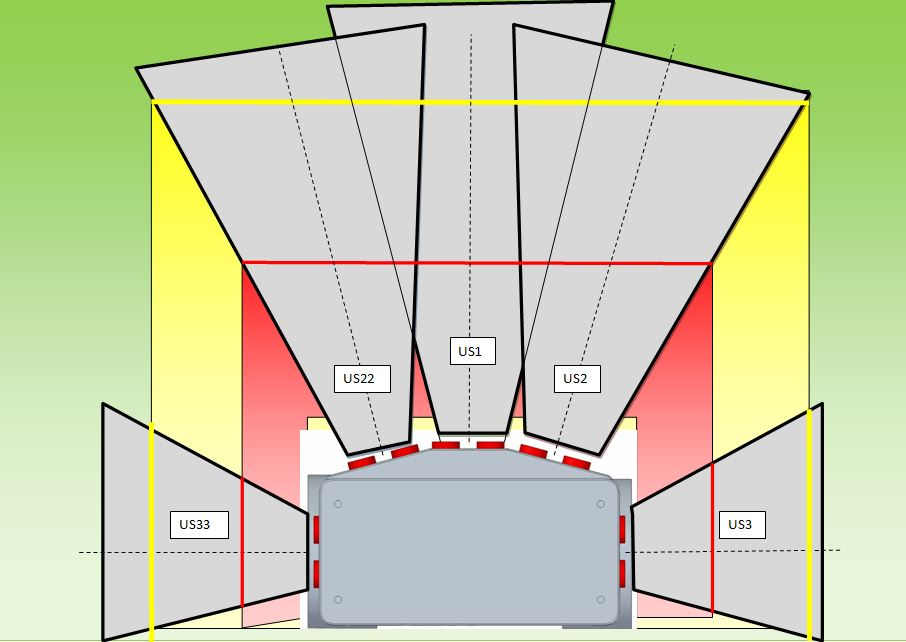
\includegraphics[width=0.85\textwidth]{images/H-UMF.jpg}
	\caption{ "Ampelsysten" zur Steuerung der Geschwindigkeit (Quelle:Eigene Darstellung)}
	\label{zone} % über das label kann man aus dem Text auf das Bild verweisen
\end{figure}

\subsection{Fallauswahl}

Es wurde unter sechs Fälle entschieden. Die alle Fälle sind auf Abbildung \ref{faelle} zu betrachten.

\begin{figure}[!h]  % [h] bedeutet, dass das Bild genau an dieser Stelle im Text erscheint
	\centering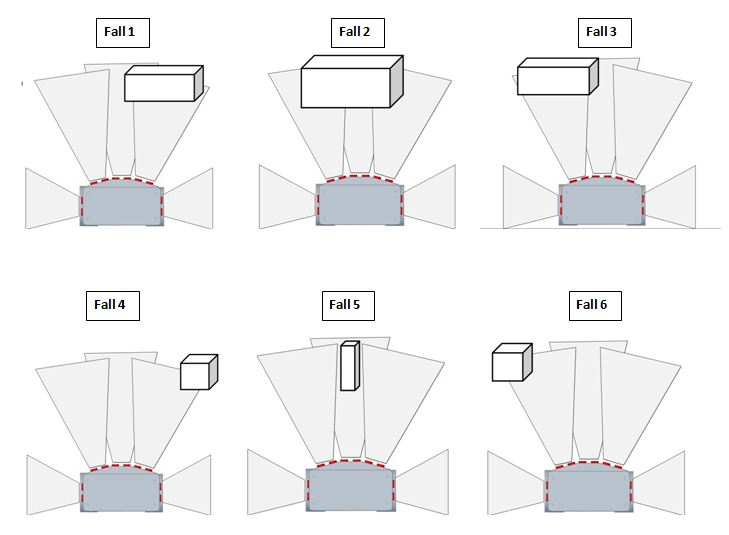
\includegraphics[width=0.7\textwidth]{images/faelle.jpg}
	\caption{ Entscheidungsmöglichkeiten (Quelle:Eigene Darstellung)}
	\label{faelle} % über das label kann man aus dem Text auf das Bild verweisen
\end{figure}

\subsection{Entscheidungsbaum}

 In diesem Fall wird in Abhängigkeit von der aktuellen Orientierung des Hindernis entschieden, wie es am günstigsten ist sich zu drehen, um das Fahren entlang des Hindernisses fortzusetzen. 
 
\begin{figure}[!h] 
	\centering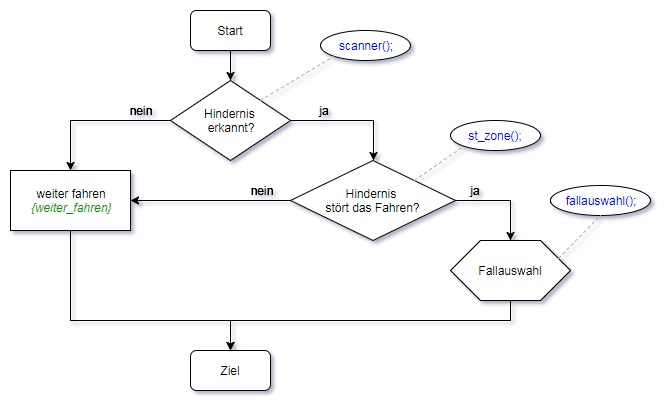
\includegraphics[width=0.75\textwidth]{images/Entsch-baum1.jpg}
	\caption{ \ Entscheidungsbaum für "Hindernis umfahren";\textcolor{blue}{\textit{scanner(); skal\_zone();}} und \textcolor{blue}{\textit {fallauswahl();}} sind Teilprogramme;   (Quelle:Eigene Darstellung)}
	\label{baum1} 
\end{figure}

Im Strukturgramm sieht man schön, wie der Roboter sich vor einem Hindernis verhalten soll. Um eine Prüfung des Hinderniserkennung zu starten muss man Zielkoordinaten eingeben. Danach fängt den Roboter scannen und die Ergebnisse zu bewerten. Für die Bewertung wurde hier wieder eine vereinfachte grafische Darstellung - Bild \ref{baum2} erstellt.

In nachfolgender Abbildung \ref{baum2} wird das Teilprogramm so lange aufgefordert ein Hindernis umzufahren, bis er nicht mehr stört.

\begin{figure}[!h]  % [h] bedeutet, dass das Bild genau an dieser Stelle im Text erscheint
	\centering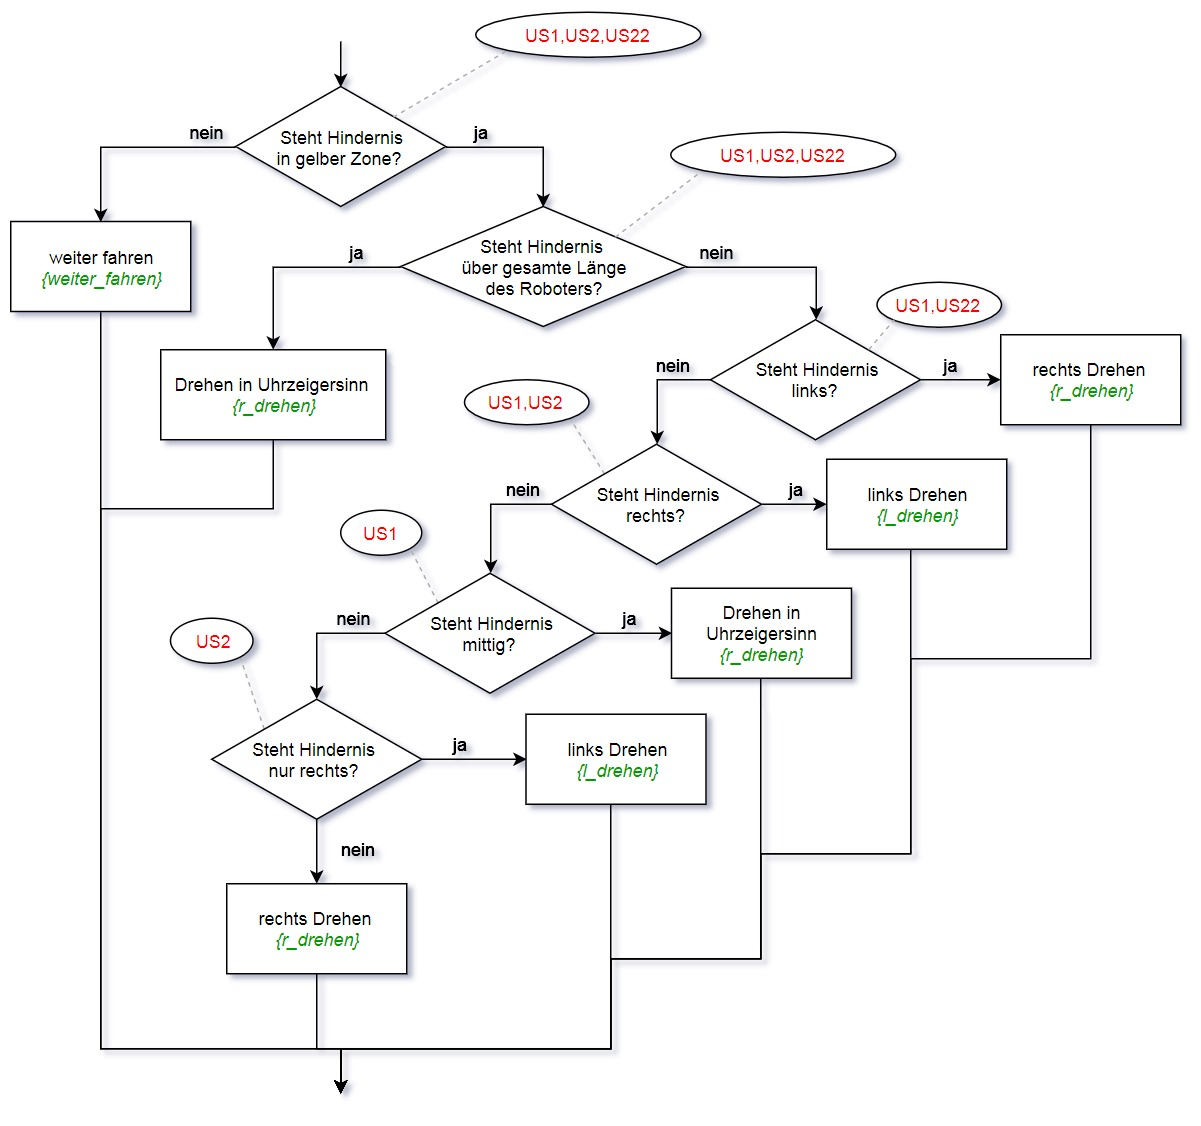
\includegraphics[width=0.99\textwidth]{images/Entsch-baum2.jpg}
	\caption{ Fallauswahl bei "Hindernis umfahren" (Quelle:Eigene Darstellung)}
	\label{baum2} % über das label kann man aus dem Text auf das Bild verweisen
\end{figure}
\pagebreak

\subsection{Arduino-Code}

Mit der Hilfe von Arduino-Uno senden man die Sensorwerte und Bewegungsverhalten an mBed-Platine. 

\begin{lstlisting}[language=C++, caption=Code zur Hinderniserkennung und Hindernif umfahren, label={lst:deadReackon}]
#include <NewPing.h>
#define Trig_Pin_33   6
#define Echo_Pin_33   7
#define Trig_Pin_22  12
#define Echo_Pin_22  13
#define Trig_Pin_1   8
#define Echo_Pin_1   9
#define Trig_Pin_2   10
#define Echo_Pin_2   11
#define Trig_Pin_3   4
#define Echo_Pin_3   5
#define Max_Distance 200

NewPing sonar1 (Trig_Pin_1, Echo_Pin_1, Max_Distance);
NewPing sonar2 (Trig_Pin_2, Echo_Pin_2, Max_Distance);
NewPing sonar22 (Trig_Pin_22, Echo_Pin_22, Max_Distance);
NewPing sonar3 (Trig_Pin_3, Echo_Pin_3, Max_Distance);
NewPing sonar33 (Trig_Pin_33, Echo_Pin_33, Max_Distance);

float skalierung;
float duration1;
float duration2;
float duration22;
float duration3;
float duration33;
float US1;                      //Sensor front middl
float US2;                      //Sensor front right
float US22;                     //Sensor front left
float US3;                      //Sensor side right
float US33;                     //Sensor side left
float soundsp;
float soundcm;
int interations = 3;

int skal_zone;            
//Skalierung zone = 1 sehr langsam / zone = 2 langsam / zone = 3 norm. fahren
int winkel;               
//bei winkel=1 färht er gerade aus./ winken=0 (minus Winkel) / winken=2 (plüs Winkel)

void sk_zone(void);
void langsam_fahren(void);
void fallauswahl(void);
void IBO_drehen(void);  
void go_drehen(void);
void l_drehen(void); 
void r_drehen(void);
void weiter_fahren(void);  
void langsam_fahren(void);   
void rueckwertsfahren(void);

void setup() {
Serial.begin(9600);
pinMode(Trig_Pin_1, OUTPUT);
pinMode(Echo_Pin_1, INPUT);
pinMode(Trig_Pin_2, OUTPUT);
pinMode(Echo_Pin_2, INPUT);
pinMode(Trig_Pin_22, OUTPUT);
pinMode(Echo_Pin_22, INPUT);
pinMode(Trig_Pin_3, OUTPUT);
pinMode(Echo_Pin_3, INPUT);
pinMode(Trig_Pin_33, OUTPUT);
pinMode(Echo_Pin_33, INPUT); }

void loop()    {
scanner();
sk_zone();
fallauswahl(); }

void scanner(){
duration1 = sonar1.ping_median(interations);
US1 = (duration1 / 2) * 0.0341;
duration2 = sonar2.ping_median(interations);
US2 = (duration2 / 2) * 0.0341;
duration22 = sonar22.ping_median(interations);
US22 = (duration22 / 2) * 0.0341;
duration3 = sonar3.ping_median(interations);
US3 = (duration3 / 2) * 0.0341;
duration33 = sonar33.ping_median(interations);  
US33 = (duration33 / 2) * 0.0341; }

void sk_zone() {  
//zone = 1 anhalten und drehen / zone = 2 langsam und abbiegen / zone = 3 norm. fahren

if ((US1 > 15 && US1 < 50)  || (US2 > 15 && US2 < 50)  || (US22 > 15 && US22 < 50) || (US3 > 10 && US3 < 30) || (US33 > 10 && US33 < 30)){
skal_zone = 1;  }
else if ((US1>2 && US1<15) || (US2>2 && US2<15) || (US22>2 && US22<15 ) || (US3>2 && US3<10) || (US33>2 && US33<10)){
skal_zone = 0;  }
else { skal_zone = 4; } }

void fallauswahl(){ 
if ((US1>2 && US1<15) || (US2>2 && US2<15) || (US22>2 && US22<15) || (US3>3 && US3<10) || (US33>3 && US33<10)) { langsam_fahren();
if ((US3>3 && US3<10) || (US33>3 && US33<10)) {
if (US3>2 && US3<10)   { l_drehen();  } 
else                   { r_drehen();  } } }
else if ( (US1>2 && US1<50) || (US2>2 && US2<50) || (US22>2 &&  US22<50)) 
{ langsam_fahren(); 
if ((US1>2 && US1<50) && (US2>2 && US2<50) && (US22>2 &&  US22<50)) 
{ go_drehen();  }
else if ((US1>2 && US1<50)  && ( US22>2 && US22<50))
{ r_drehen();   }
else if ((US1>2 && US1<50) && (US2>2 && US2<50))  { l_drehen();   }
else if (US1>2 && US1<50)                 { r_drehen();   }
else if (US2>2 && US2<50)                 { l_drehen();   }
else                                      { r_drehen();   } }
else                                      { weiter_fahren(); } }

void langsam_fahren(){   
winkel = 0;
Serial.write(skal_zone);
Serial.write(winkel);
Serial.println(); }

void weiter_fahren(){   
winkel = 0;
Serial.write(skal_zone);
Serial.write(winkel);
Serial.println(); }

void r_drehen(){ 
winkel = -2;
Serial.write(skal_zone);
Serial.write(winkel);
Serial.println(); }

void l_drehen(){ 
winkel = 2;
Serial.write(skal_zone);
Serial.write(winkel);
Serial.println(); }

\end{lstlisting}

\pagebreak